\documentclass[12pt]{article}

% Page format
\usepackage[margin=1in]{geometry}

% Math packages and custom commands 
\usepackage{framed, tikz}
\usepackage[utf8]{inputenc}
\usepackage{mathtools,amsthm}
\usepackage{enumitem,amssymb}
\usepackage{hyperref}

\newtheoremstyle{case}{}{}{}{}{}{:}{ }{}
\theoremstyle{case}
\newtheorem{case}{Case}
\DeclareMathOperator{\R}{\mathbb{R}}
\DeclareMathOperator{\E}{\mathbb{E}}
\DeclareMathOperator{\Var}{\text{Var}}
\DeclareMathOperator{\Cov}{\text{Cov}}
\newcommand{\bvec}[1]{\mathbf{#1}}
\renewcommand{\P}{\mathbb{P}}
\newcommand{\norm}[2][2]{\| #2\|_{#1}}
\newcommand{\maxnorm}[2][\infty]{\| #2\|_{#1}}
\newcommand{\note}[1]{\noindent{[\textbf{NOTE:} #1]}}
\newcommand{\hint}[1]{\noindent{[\textbf{HINT:} #1]}}
\newcommand{\recall}[1]{\noindent{[\textbf{RECALL:} #1]}}

\definecolor{shadecolor}{gray}{0.9}


\begin{document}

\begin{center}
{\Large CSCE 580, Fall 2020 \\ Assignment 4}

\begin{tabular}{rl}
Username: & Primiani \\
Name: & Jack Primiani \\
\end{tabular}
\end{center}

By turning in this assignment, I agree by the honor code of USC Columbia.

\paragraph{Submission.}
You need to submit the following file to Blackboard:
\begin{itemize}
    \item A pdf file named as assignment4\_$\langle username \rangle$.pdf, where you replace $\langle username \rangle$ with your email username. This pdf file contains your answers to all the problems below: Edit the assignment4.tex file to fill in your answers for the problems, and submit the pdf file generated from the edited tex file. 
\end{itemize}

\section*{Problem 1 [25 pt]}
Futoshiki is a Japanese logic puzzle that is very simple, but can be quite challenging. You are given an $n \times n$ grid, and must place the numbers $1,...,n$ in the grid such that every row and column has exactly one of each. Additionally, the assignment must satisfy the inequalities placed between some adjacent squares.

The figure below is an instance of this problem, for size $n = 4$. Some of the squares have known values, such that the puzzle has a unique solution. (The letters mean nothing to the puzzle, and will be used only as labels with which to refer to certain squares). Note also that inequalities apply only to the two adjacent squares, and do not directly constrain other squares in the row or column.

Let’s formulate this puzzle as a CSP. We will use $4^2$ variables, one for each cell, with $X_{ij}$ as the variable for the cell in the $i$th row and $j$th column (each cell contains its $i,j$ label in the top left corner). The only unary constraints will be those assigning the known initial values to their respective squares, i.e. $X_{34} = 3$ and $X_{43}=2$.


\begin{figure}[h]
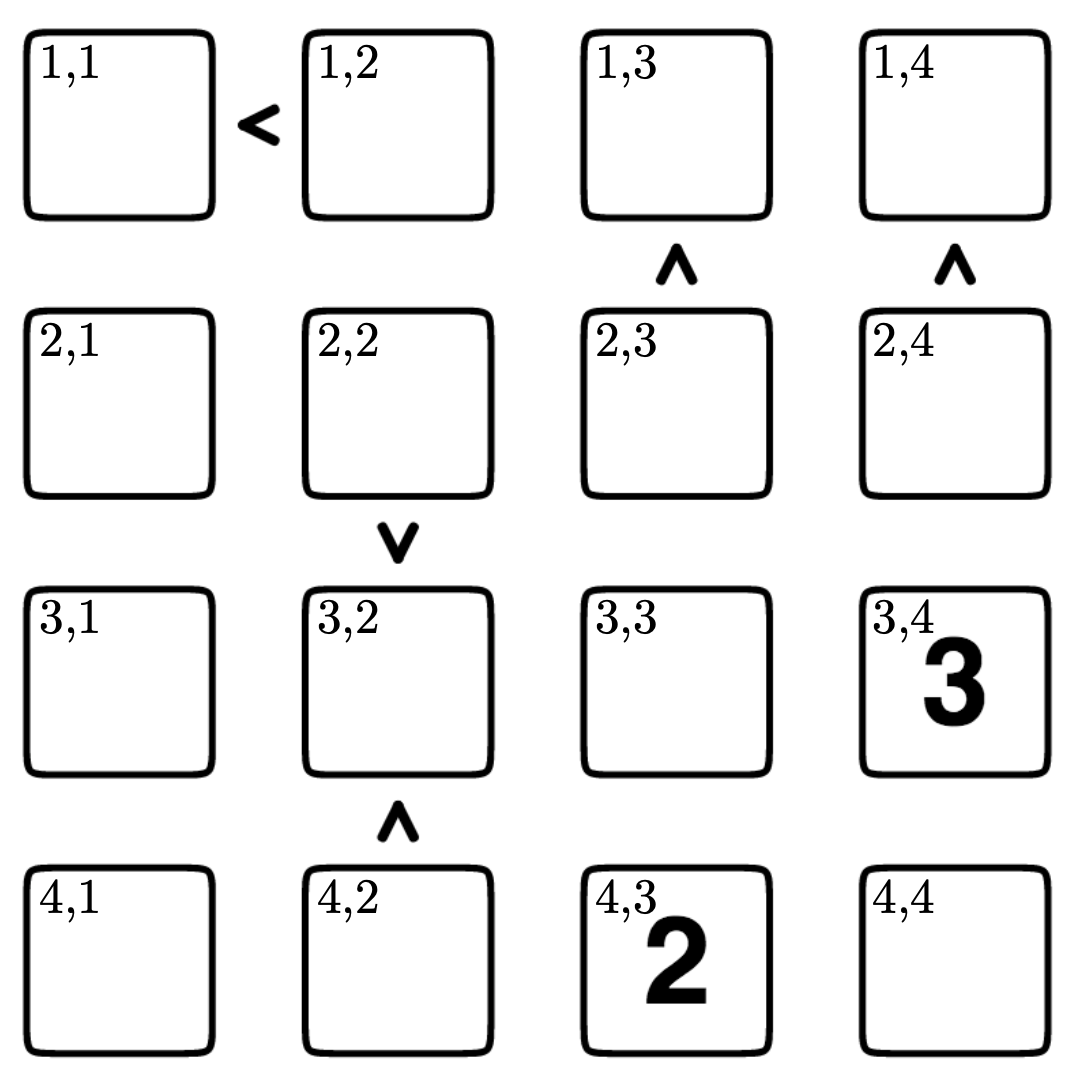
\includegraphics[width=.37\textwidth]{assignment4_1.png}
\centering
\end{figure}
 
    
\begin{enumerate} [label=(\alph*)]
    \item
    Complete the formulation of the CSP using only binary constraints (in addition to the unary constraints specified above. In particular, describe the domains of the variables, and all binary constraints you think are necessary. You do not need to enumerate them all, just describe them using concise mathematical notation. You are not permitted to use $n$-ary constraints where $n \geq 3$.
   
Domains:  $X_{ij} \in \{1, 2, 3, 4\}$, $\forall$i, j

Unary constraints: $X_{34}$ = 3, $X_{43}$ = 2

Inequality binary constraints: $X_{11} < X_{12}$, $X_{13} < X_{23}$, $X_{14} < X_{24}$, $X_{32}< X_{22}$, $X_{32}< X_{42}$

Row binary contraints:  $X_{ij} \neq X_{ik}$, $\forall$i, j, k, j $\neq$ k

Column binary contraints:  $X_{ij} \neq X_{kj}$, $\forall$i, j, k, i $\neq$ k


    \item 
    After enforcing unary constraints, consider the binary constraints involving $X_{14}$ and $X_{24}$. Repeatedly enforce arc consistency on just these constraints and state the resulting domains for the two variables.

    
$X_{14} \in \{1, 2\}$
$X_{24} \in \{2, 4\}$
Both threes are removed from the column constraint with $X_{34}$.


    
    \item
    By inspection of column 2, we find it is necessary that $X_{32} = 1$, despite not having found an assignment to any of the other cells in that column. Would running arc consistency find this requirement? Explain why or why not.
    
No, arc consistency would not find this requirement. Encorcing the $X_{34} \rightarrow X_{42}$ and the $X_{42} \rightarrow X_{43}$ arc leaves $X-{42}$ with a domain of $\{3, 4\}$. Enforcing the $X_{32} < X_{22}$ constraints leaves $X_{32} \in \{1, 2, 3\}$ and $X_{22} \in \{2, 3, 4\}$. Enforcing that they are all different does not remove any values. After this point, every arc in this column is consistent and $X_{32}$ is not required to be 1.
   
\end{enumerate}

\newpage
\section*{Problem 2 [25 pt]}
Let's consider a simple CSP with 3 variables and 2 binary factors:
\begin{figure}[h]
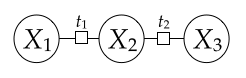
\includegraphics[width=.3\textwidth]{assignment4_2.png}
\centering
\end{figure}

where $X_1, X_2, X_3 \in \{0,1\}$ and $t_1$, $t_2$ are \href{https://en.wikipedia.org/wiki/Exclusive_or}{XOR} functions.

\begin{enumerate} [label=(\alph*)]
    \item
    How many consistent assignments are there for this CSP? What are they?

There are 2 consistent assignments, $\{1, 0, 1\}$ and $\{0, 1, 0\}$.
    
    \item
    To see why variable ordering is important, let's use backtracking search to solve the CSP without using any heuristics (MCV, LCV, AC-3) or lookahead.How many times will backtrack() be called to get the first consistent assignment if we use the fixed ordering $X_1, X_3, X_2$? Draw the call stack until getting the first consistent assignment is found. (You should use the Backtrack algorithm from the slides. The initial arguments are $x=\empty$, $w=1$, and the original Domain. You can also implement the algorithm in code to help you answer this and the next questions.)
    
Backtrack will be called 9 times. The call stack is:

$\{[0,1],[0,1],[0,1]\}$


                           $x_{1}$ =0 $\rightarrow \{0, [0,1],[0,1]\}$

                           $x_{3}$ =0 $\rightarrow \{0, [0,1], 0\}$

                           $x_{3}$ =1 $\rightarrow \{0, [0,1], 1\}$

                           $x_{2}$ =1 $\rightarrow \{0, 1, 0\}$

                           $x_{1}$ =1 $\rightarrow \{1, [0,1],[0,1]\}$

                           $x_{3}$ =0 $\rightarrow \{1, [0,1], 0\}$

                           $x_{3}$ =1 $\rightarrow \{1, [0,1], 1\}$

                           $x_{2}$ =0 $\rightarrow \{1, 0, 1\}$
    
    \item
    To see why lookahead can be useful, let's do it again with the ordering $X_1, X_3, X_2$ and AC-3. How many times will backtrack() be called to get the first consistent assignment? Draw the call stack until getting the first consistent assignment is found.

Backtrack will only be called 7 times. The call stack:

{[0,1],[0,1],[0,1]} 


                           $x_{1}$ =0 $\rightarrow \{0, [1], [0]\}$

                           $x_{3}$ =0 $\rightarrow \{0, [1], 0\}$

                           $x_{2}$ =1 $\rightarrow \{0, 1, 0\}$


                           $x_{1}$ =1 $\rightarrow \{1, [0], [1]\}$

                           $x_{3}$ =1 $\rightarrow \{1, [0], 1\}$

                           $x_{2}$ =0 $\rightarrow \{1, 0, 1\}$
   
\end{enumerate}

\newpage
\section*{Problem 3 [25 pt]}

\begin{figure}[h]
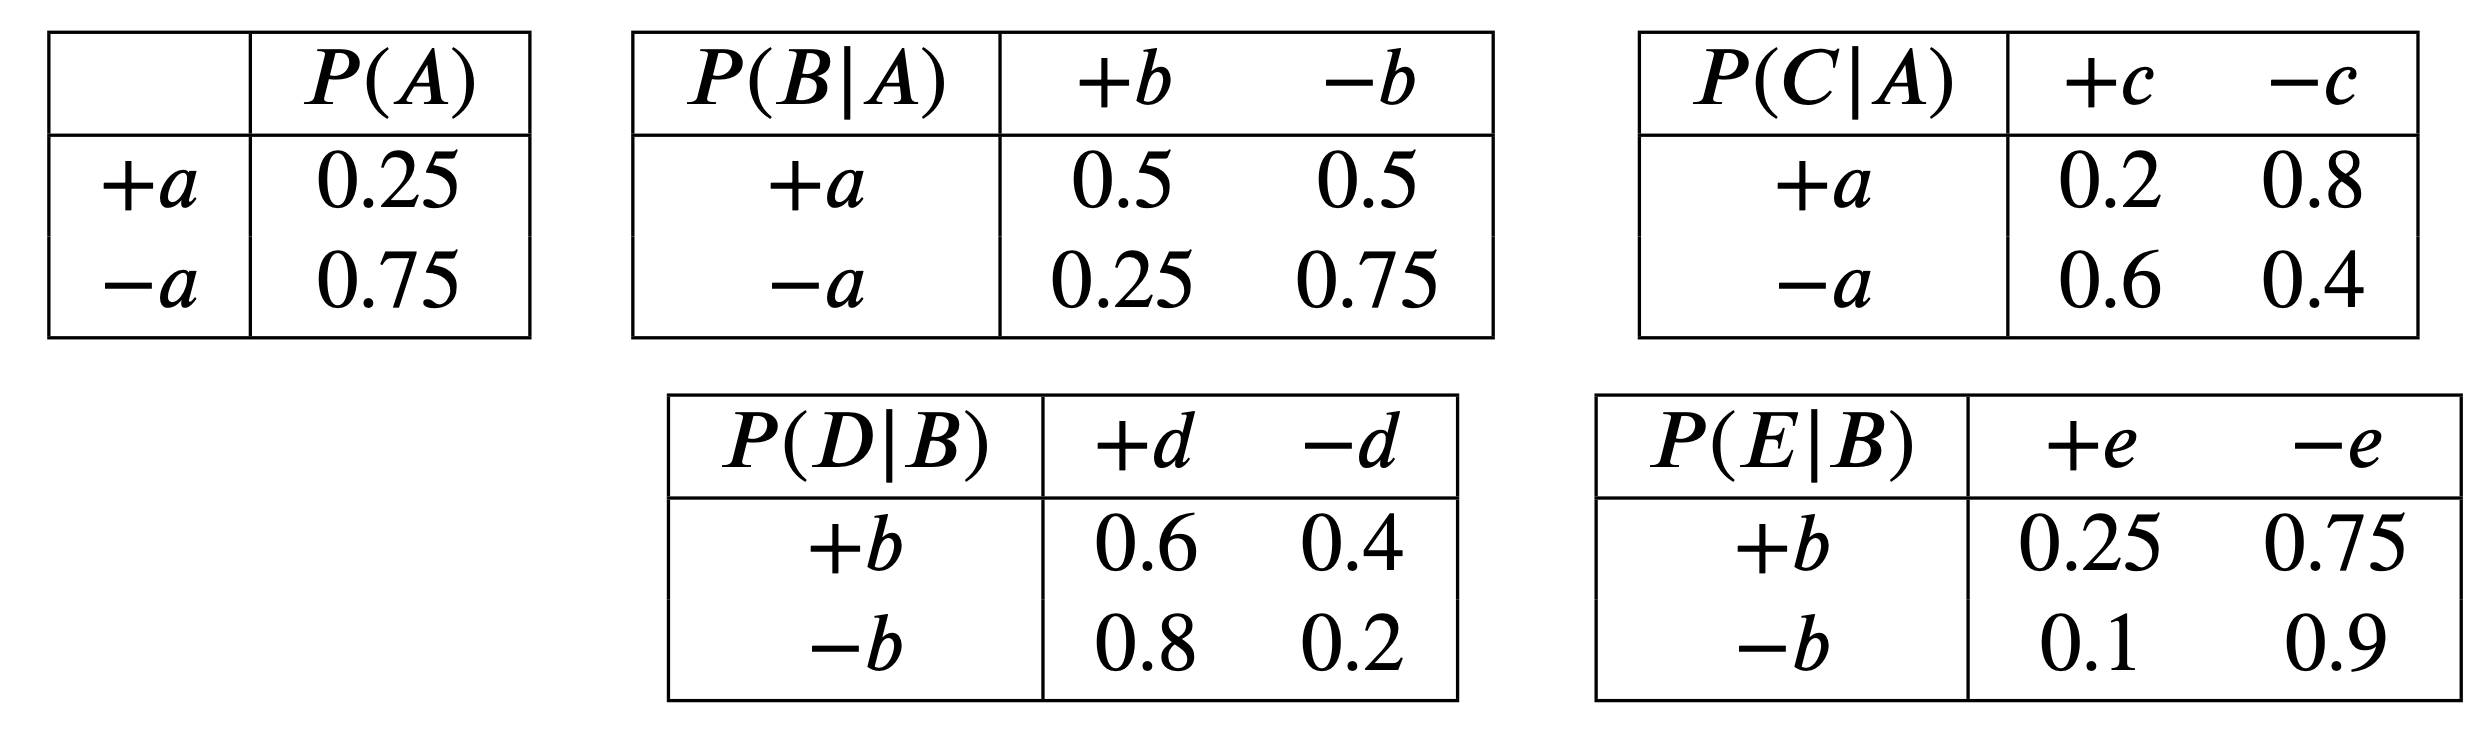
\includegraphics[width=.67\textwidth]{assignment4_3.png}
\centering
\end{figure}

Use the Bayesian network and conditional probability tables above.

\begin{enumerate} [label=(\alph*)]
\item Calculate the following quantities:
$P(+a, +b)$, $P(+a | +b)$.

0.25 * 0.5 = 0.125 = 1/8

\end{enumerate}

For the questions below, we consider variable elimination in the Bayesian network.

\begin{enumerate} [label=(\alph*)]\setcounter{enumi}{1}
\item Assume we have the evidence $+c$ and wish to calculate $P(E|+c)$. What factors do we have initially?

$P(A), P(B | A), P(+c | A), P(D | B), P(E | B)$

\item What is the equation to calculate the factor we create when eliminating variable $B$?

$f(A, D, E) = \sum_{B} P(B | A) * P(D | B) * P(E | B)$

\item After eliminating variable $B$, what are the new set of factors? For each factor, also provide its size.

P(A) size=2

$P(+c|A)$ size=2

$P(D, E | A)$ size=$2^{3}$

\item Now assume we have the evidence $-c$ and are trying to calculate $P(A|-c)$. What is the most efficient elimination ordering? If more than one ordering is most efficient, provide any one of them. 

E, D, B or D, E, B

\item Once we have run variable elimination and have $f(A, -c)$ how do we calculate $P(+a|-c)$? (give an equation)

$f(+a,-c)/(f(+a,-c)+f(-a,-c))$

\end{enumerate}

\newpage
\section*{Problem 4 [25 pt]}
\begin{figure}[h]
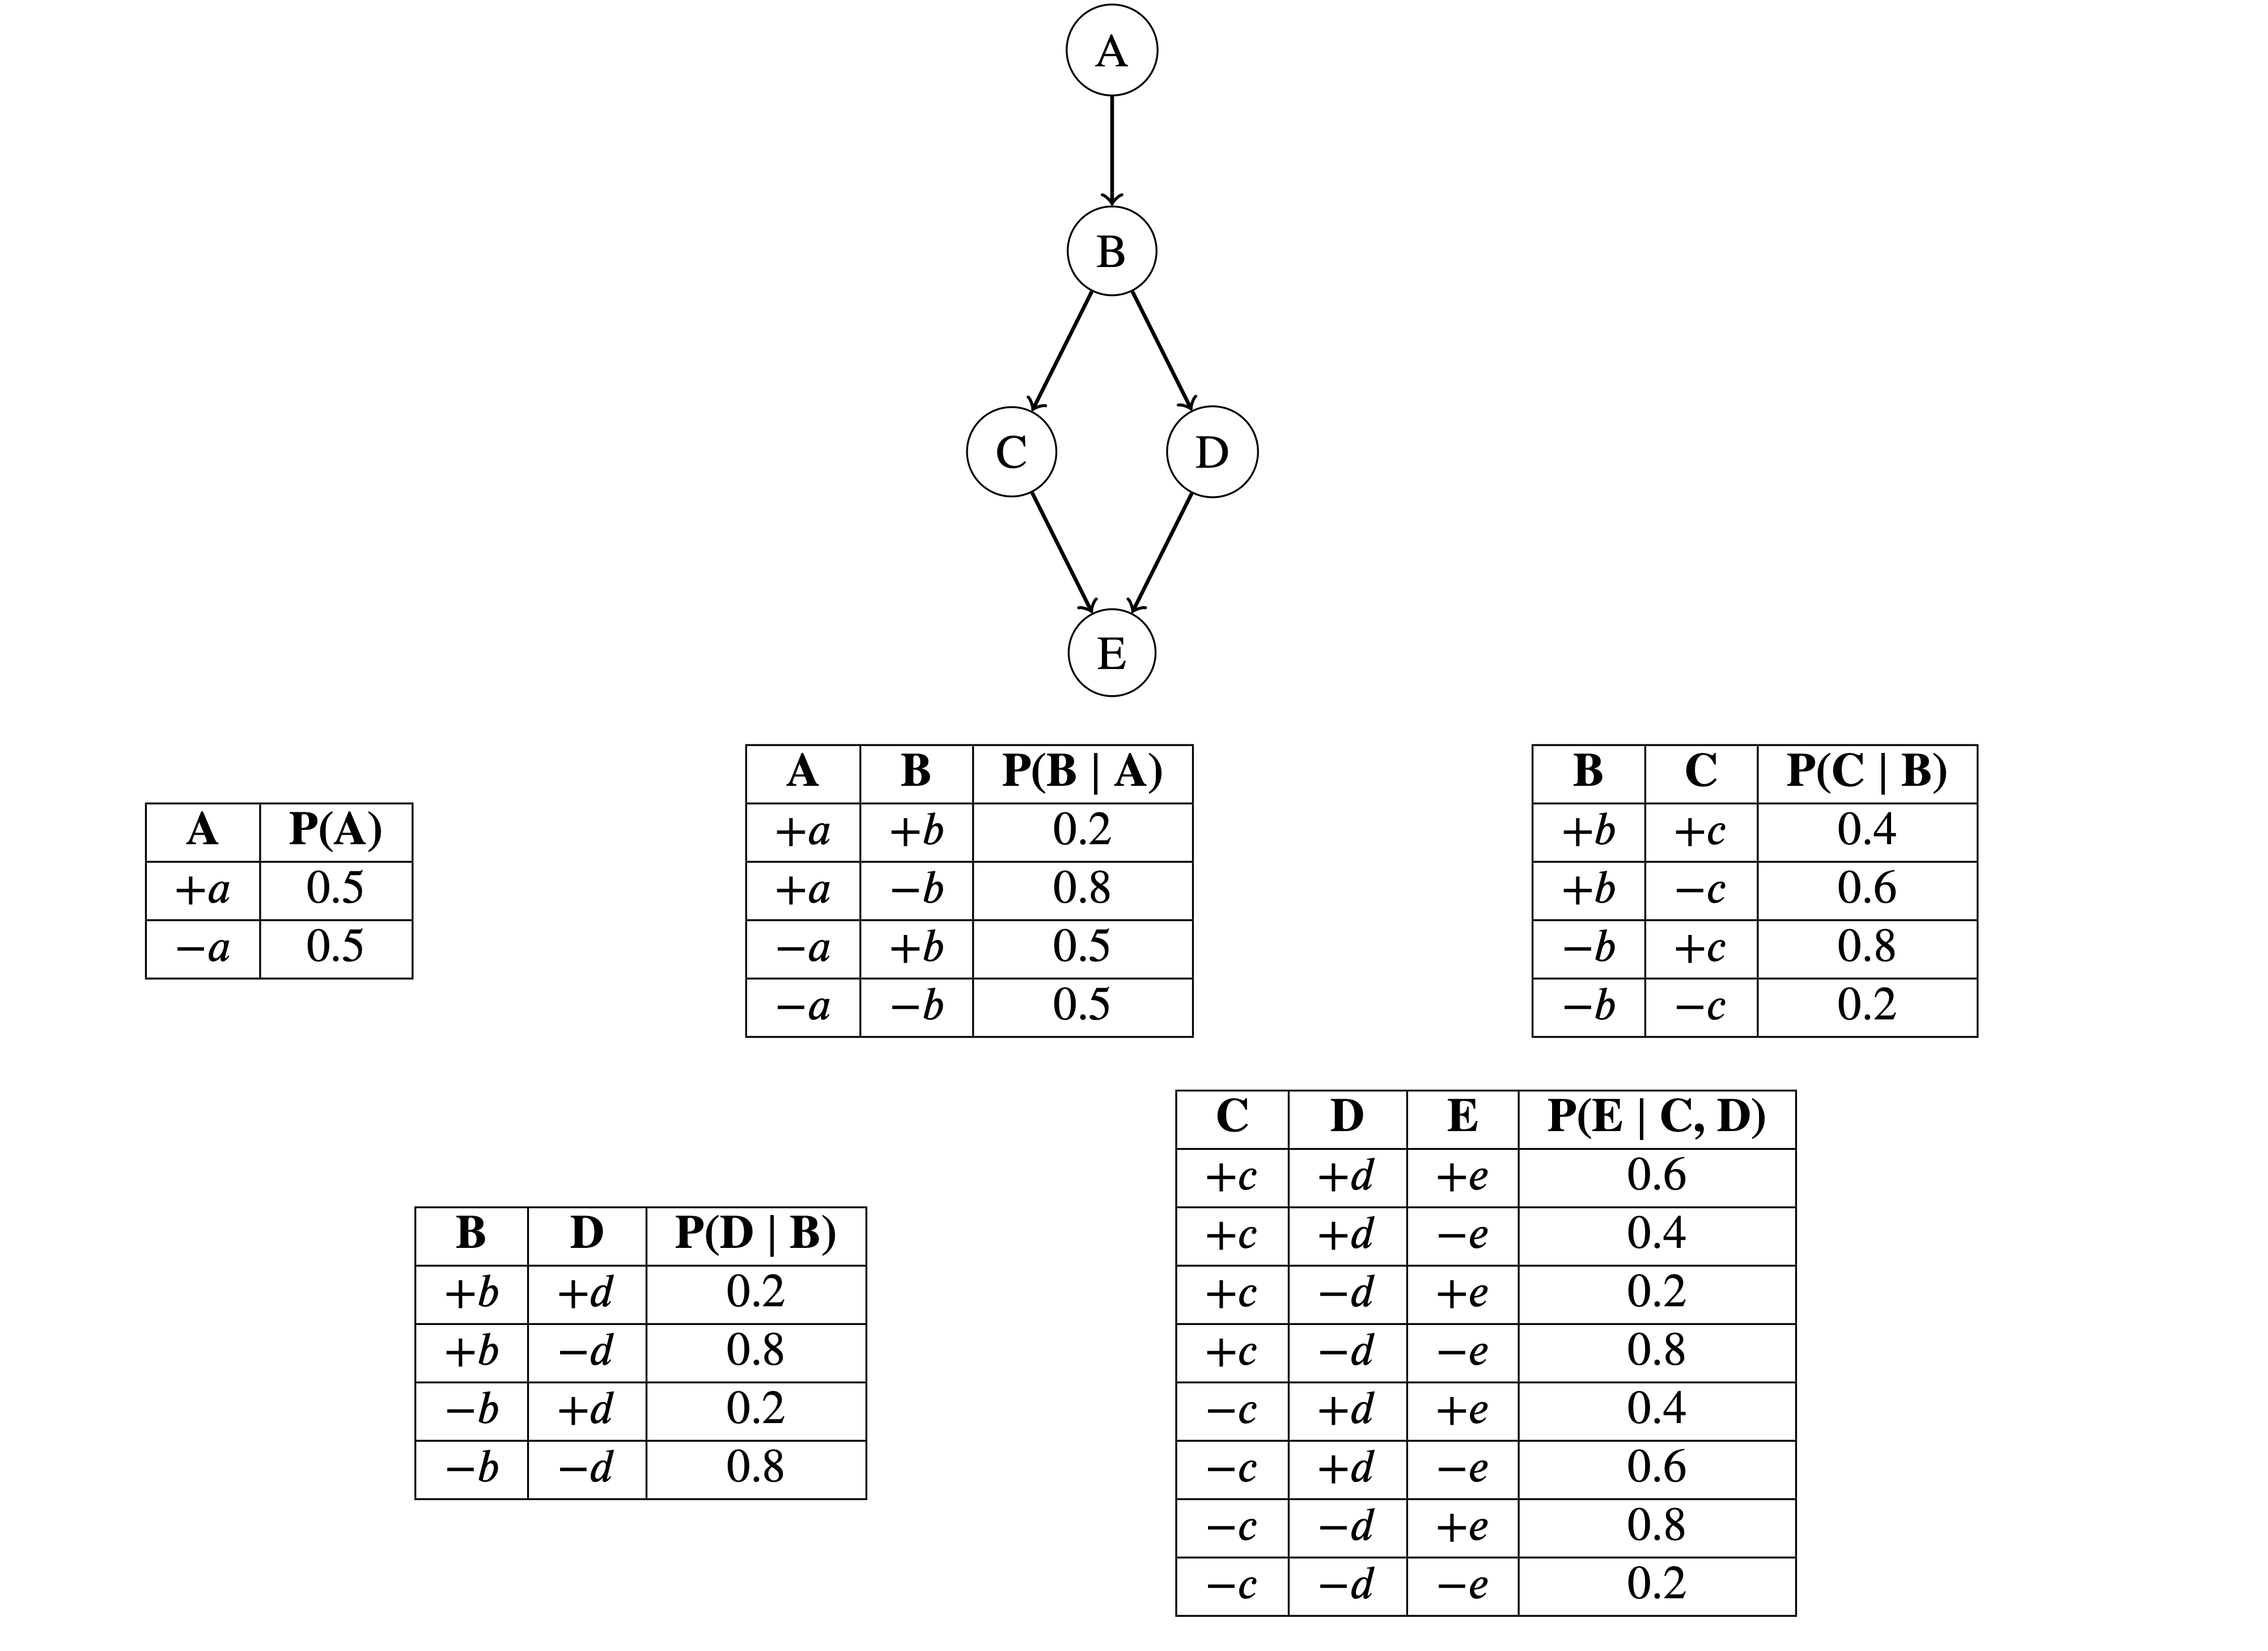
\includegraphics[width=.97\textwidth]{assignment4_4.png}
\centering
\end{figure}
Assume we are given the above Bayes’ net, with the associated conditional probability tables. Throughout this problem, you may answer as either numeric expressions (e.g. $0.1 * 0.5$) or numeric values (e.g. $0.05$).

For questions (a) and (b), you are given a set of the following samples, but are not told whether they were collected with rejection sampling or likelihood weighting.
\begin{align*}
-a \quad -b \quad +c \quad +d \quad +e \\
-a \quad +b \quad +c \quad -d \quad +e \\
-a \quad -b \quad -c \quad -d \quad +e \\
-a \quad -b \quad +c \quad -d \quad +e \\
-a \quad +b \quad +c \quad +d \quad +e
\end{align*}

\begin{enumerate} [label=(\alph*)]
\item Assuming these samples were generated from rejection sampling, what is the sample based estimate of $P(+b|-a, +e)$? Show your steps of the calculation.

The answer is the number of samples satisfying the query variable’s assignment (in this case, B = +b divided by the total number of samples, so the answer is 2 / 5 = 0.4.

\item
Assuming these samples were generated from likelihood weighting,what is the sample-based estimate of $P(+b|-a, +e)$? Show your steps of the calculation.

The weight of each sample is P(A = a) * P(E = e | C = c, D = d). 

The weights are: 0.3 (= 0.5 * 0.6), 0.1 (= 0.5 * 0.2), 0.4 (= 0.5 * 0.8), 0.1 (same assignments to C and D as second sample), 0.3 (same assignments to C and D as first sample). 

The estimate is then (0.1 + 0.3) / (0.3 + 0.1 + 0.4 + 0.1 + 0.3) = 0.4 / 1.20 = 1/3 = 0.333.

\end{enumerate}

For the questions below, suppose you choose to use Gibbs sampling to estimate $P(B,E|+c, -d)$. Currently the assignment is the following:
\begin{align*}
    -a \quad -b \quad +c \quad -d \quad +e
\end{align*}
\begin{enumerate} [label=(\alph*)]\setcounter{enumi}{2}
\item Suppose the next step is to resample $E$. What is the probability that the new assignment to $E$ will be $+e$?

Calculate P(E | -a, -b, +c, d), which is equal to P(E | +c, -d) since E is conditionally independent of A and B, given C and D. The value for P(+e | +c, -d) is given directly in the CPT for P(E|C, D), and it is 0.2.

\item Instead, suppose the next step is to resample $A$. What is the probability that the new assignment to $A$ will be $+a$?

Calculate P(A | -b, +c, -d, +e), which is equal to P(A | B) since A is conditionally independent of C, D, and E, given B.  This can be calculated with Bayes Rule

(0.8*0.5)/(0.8*0.5+0.5*0.5) = 0.4/0.65 = 8/13

\end{enumerate}

\end{document}